\documentclass[conference]{IEEEtran}

\usepackage{cite}
\usepackage{amsmath,amssymb,amsfonts}
\usepackage{algorithmic}
\usepackage{graphicx}
\usepackage{textcomp}
\usepackage{xcolor}
\def\BibTeX{{\rm B\kern-.05em{\sc i\kern-.025em b}\kern-.08em
    T\kern-.1667em\lower.7ex\hbox{E}\kern-.125emX}}
\begin{document}

\title{TODO - Come up with cool title\\}

\author{\IEEEauthorblockN{1\textsuperscript{st} Given Name Surname}
\IEEEauthorblockA{\textit{dept. name of organization (of Aff.)} \\
\textit{name of organization (of Aff.)}\\
City, Country \\
email address}
\and
\IEEEauthorblockN{2\textsuperscript{nd} Given Name Surname}
\IEEEauthorblockA{\textit{dept. name of organization (of Aff.)} \\
\textit{name of organization (of Aff.)}\\
City, Country \\
email address}
\and
\IEEEauthorblockN{3\textsuperscript{rd} Given Name Surname}
\IEEEauthorblockA{\textit{dept. name of organization (of Aff.)} \\
\textit{name of organization (of Aff.)}\\
City, Country \\
email address}
}

\maketitle

\begingroup
    \begin{abstract}
    In this paper, we analyze the performance of DNS over different internet protocols in an effort to compare the performance of the protocols and examine how well the experimental HTTP/3 performs.  Using Google Compute Engine, many virtual machines spanning the globe were instantiated to run our experiment and collect data. In each region offered by Google Compute, there were three virtual machine instances where each had a specific simulated network type. Using multiple vantage points and simulated networks gave depth to the data and comparisons by showing the performance of DNS over specific internet protocols for different locations with a high-grade, mid-grade, and low-grade simulated network connection. HTTP/3 boasts its speed and encryption; however, given the results it may not be the highest performing protocol in terms of time, but the trade-off could be the extra security provided by its encryption.
\end{abstract}
\endgroup%

\begingroup
    \section{Introduction}
The goal of this research effort was to compare the performance of DNS over multiple different protocols and ultimately compare them to HTTP/3.  The protocols used in the experiment were HTTP/1.0, HTTP/1.1, HTTP/2, HTTP/3, TLS1.0, TLS1.2, TLS1.3, and traditional DNS. These were chosen to give a broad scope of comparison and demonstrate the performance of popularly used protocols to the experimental HTTP/3. The HTTP/3 protocol is under consideration to become an internet standard, and is already being used by some popular internet companies such as Google.  There are also libraries that support the protocol in popular programming languages like Python, Rust, and C.  HTTP/3 boasts faster speeds and performance through the use of UDP and is also referred to as HTTP-over-QUIC where QUIC stands for “Quick UDP Internet Connections”.  Taking advantage of the already existing lower-level UDP protocol, HTTP/3 could be implemented without having to upgrade kernels of internet systems.  UDP is also not constrained by single data streams like TCP; one data stream failure does not have to impact the others.  The aim of the experiment was to gather timing data from various vantage points using multiple internet protocols resolving a DNS request.  The timing data was utilized for a comparison between the protocols.  It was found that HTTP/3 did not have any substantial performance improvements to the timings of the current protocols, but the difference could be miniscule when HTTP/3 might be effective for extremely poor internet connections or provide extra security.
\endgroup%

\begingroup
    \section{Experimental Setup}
The objective of the experiment was to collect timing performance data for resolving DNS queries over chosen protocols and ultimately compare them to the experimental performance of DNS-over-HTTP/3.  In order to analyze performance between DNS-over-HTTP/3 and other various protocols, a software package was built to make the appropriate timing measurements for http/3, http/2, http/1.1, http/1.0, tls1.3, tls1.2, tls1.0, and traditional dns. The measurements were evaluated for Google and Cloudflare DNS servers, as both support the http/3 protocol for resolving dns queries [7,8].  The software package included industry standard tools, with curl being the most important to support all the protocols mentioned above. In order to fully support experimental http/3, curl was built from source and had to have an implementation of a QUIC transport protocol, and in this case, Quiche was the implementation that was chosen \cite{curl,quiche}.  To get samples for traditional DNS, kdig was the tool selected [3].  A build script was used to install package dependencies, clone the required repos, and build the tools that were needed for this experiment. At the end of the build script, a cronjob was initialized to run the data collection script every 15 minutes over the course of an entire week, with the experiment being completed at the end of that time period.  The data collection script would perform the curl, kdig, ping, and traceroute commands and pipe the output into respective text files. The commands resolved Amazon’s URL and collected timing data for name lookup, connection, app connection, pre-transfer, redirect, start transfer, and time total [6].  Once the experiment was completed, a cleanup script would run that would uninstall any packages the build script had to install, as well as remove the built software tools and remove the cronjob. 
Initially, the software package was sent to volunteers to run on their personal machines. The only requirement for users to be able to run the software package was to have a machine with a distribution of Linux or Mac operating systems. Only a few participants could be sourced to run the experiment and they all resided in the same county in North Alabama. This gave data for a small geographical area and did not add depth to the data as there was no variation in networks or locations. As a next step to broaden our data collection vantage points, Google Compute Engine virtual machines were utilized [4].  Since the virtual machines are a part of a well constructed computing network, the addition of Linux traffic shaping was added to the experiment setup to simulate three types of network: a high-grade, mid-grade, and low-grade network defined in Table 1.  Three virtual machines were instantiated in each region that Google Compute Engine offered (one for each type of network) and the experiment was run on each for data collection; the regions are shown in Figure A.
\begin{figure}[htpb]
    \centering
    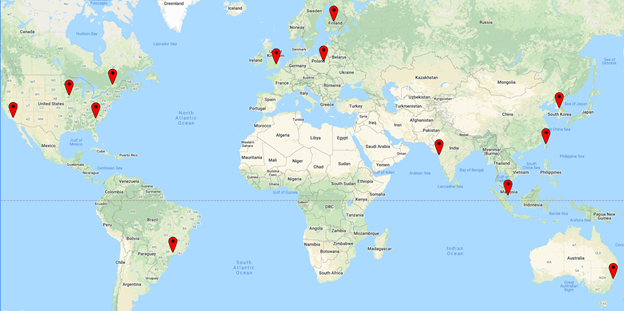
\includegraphics[width=8cm]{figures_and_tables/map.png}
    \caption{Fig. A. The locations for the virtual machines: California, Iowa, South Carolina, Canada, Brazil, England, Poland, Finland, India, Singapore, Taiwan, South Korea, Australia [5]}
    \label{fig:map}
\end{figure}
\endgroup%

\begingroup
    \section{Results and Analysis}
Todo
\endgroup%

\begingroup
    \section{Issues and Future Work}
When running the experiment, there were some issues experienced with the Cloudflare DNS resolver.  Cloudflare was used because it was a second server along with Google that supported HTTP/3.  The first issue was Cloudflare’s HTTP/3 support was down temporarily.  This delayed the data collection for the experiment.  The second issue was found when graphing hourly data for DNS-over-HTTP/3 for the Cloudflare server.  The graph displayed a few anomalies in the timing data and it was discovered the timings for these large spikes in time were the timeout for the curl command.  The experiment was run again to test for more anomalies, but none were found the second time.  The reasoning for the timeouts is unknown and could be due to running the experiment shortly after HTTP/3 support came online and it needed further maintenance.  Outside of the Cloudflare issues, the data for DNS-over-HTTP/3 was initially surprising.  It was expected that it would be substantially faster than the other protocols, but that was not the case.  The protocol is still under development and can further be improved on, so while it is not the quickest currently it has potential to be improved upon.
\endgroup%

\begingroup
    \section{Conclusion}
Todo
\endgroup%

\section*{Acknowledgment}
Todo

\bibliographystyle{./bibliography/IEEEtran}
\bibliography{./bibliography/References}

\vspace{12pt}
\color{red}
IEEE conference templates contain guidance text for composing and formatting conference papers. Please ensure that all template text is removed from your conference paper prior to submission to the conference. Failure to remove the template text from your paper may result in your paper not being published.

\end{document}
